\documentclass{beamer}
\usepackage{graphicx}
\usepackage{alltt}

\begin{document}

\begin{frame}
 \frametitle{Hello}
 Welcome to the end of PCS!

 (As brought to you by Alyssa and Ilias.)
\end{frame}

\begin{frame}
 \frametitle{CUDA!}
\end{frame}

\begin{frame}[fragile]
 \frametitle{CUDA is easy?}
\begin{verbatim}
cudaMalloc(&d_src, sizeof(double) * w * h);

...

cudaMemcpy(d_dst, dst,
  sizeof(double) * w * h,
  cudaMemcpyHostToDevice);

...

do_calc<<<blockSize, threadSize>>>(d_c,
  d_src, d_dst, w, h);
do_smear<<<h-2, 1>>>(d_dst, w, h);
\end{verbatim}
\end{frame}

\begin{frame}[fragile]
 \frametitle{CUDA is easy!}
\begin{verbatim}
void __global__ do_calc(double *c, double *src,
  double *dst, size_t w, size_t h)
{
  unsigned x = blockIdx.x * blockDim.x
    + threadIdx.x + 1;
  unsigned y = blockIdx.y * blockDim.y
    + threadIdx.y + 1;
  ...
\end{verbatim}
\end{frame}

\begin{frame}[fragile]
 \frametitle{Xeon Phi: offloading}
\begin{verbatim}
#pragma offload_transfer target(mic)
  in(c,src,dst:length(w*h)
  alloc_if(1) free_if(0))

/* compute */
#pragma offload target(mic)
  in(c,src,dst:length(0)
  alloc_if(0) free_if(0))
#pragma omp parallel for
\end{verbatim}
\end{frame}

\begin{frame}[fragile]
 \frametitle{Xeon Phi: reductions}
\begin{verbatim}
// iterate over non-constant rows
#pragma offload target(mic)
  inout(tmin, tmax, maxdiff, tavg)
  in(src,dst:length(0)
  alloc_if(0) free_if(0))
#pragma omp parallel for
  reduction(min: tmin) ...

\end{verbatim}
\end{frame}


\begin{frame}
 \frametitle{Xeon Phi: awesome?}
 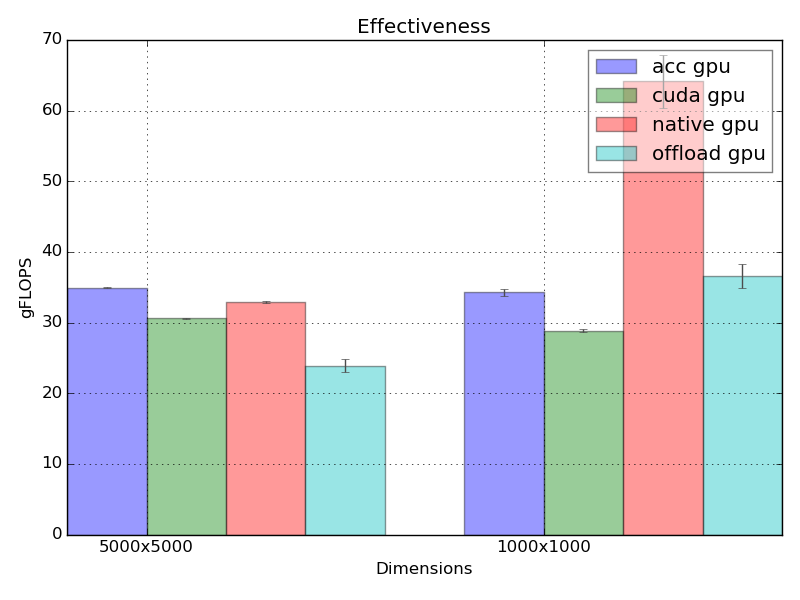
\includegraphics[width=\textwidth]{bonus_effectivness.png}
\end{frame}

\begin{frame}
 \frametitle{Xeon Phi: fail}
 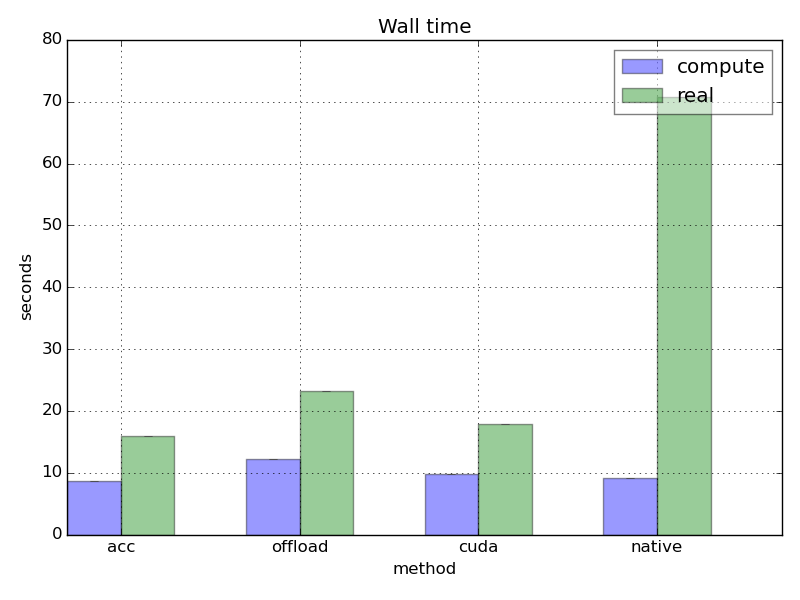
\includegraphics[width=\textwidth]{bonus_realvscompute.png}
\end{frame}

\begin{frame}
 \frametitle{Interlude}
 Did anyone try the other sub-assignments?
\end{frame}

\begin{frame}
 \frametitle{Chapel}
 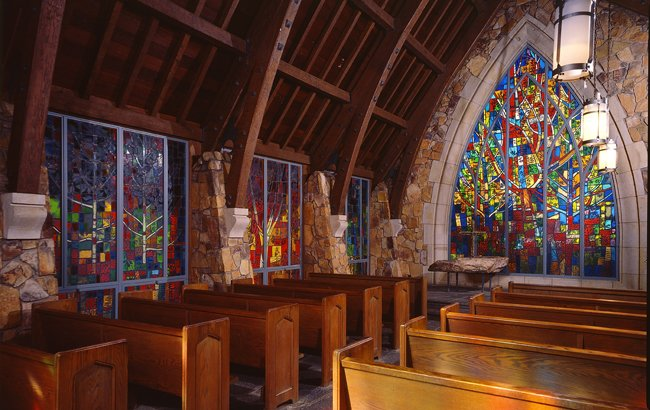
\includegraphics[width=\textwidth]{chapel.jpg}
\end{frame}
 
\begin{frame}
 \frametitle{Chapel: Happy Christmas!}
 
\includegraphics[width=\textwidth]{chrcha.jpg}
\end{frame}

\begin{frame}[fragile]
 \frametitle{Chapel}
\begin{verbatim}
[amilburn@fs0 cpl]$ make heat
\end{verbatim}
\end{frame}

\begin{frame}
 \frametitle{Chapel compiles}
 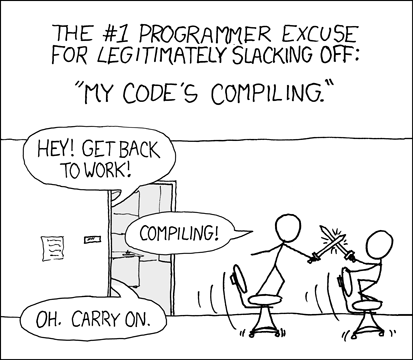
\includegraphics[width=0.8\textwidth]{xkcd.png}
\end{frame}

\begin{frame}[fragile]
 \frametitle{Chapel: why so slow?}
\begin{verbatim}
$ chpl -o heat --fast --print-passes main.chpl
  common.chpl compute.chpl
Pass               Name                  Time
---- ---------------------------------  ------
  42 makeBinary                          77.7
  13 resolve                              6.4
  41 codegen                              2.1
   6 scopeResolve                         1.7
  29 copyPropagation                      1.4
\end{verbatim}
\end{frame}

\begin{frame}[fragile]
 \frametitle{Chapel: why so slow?}
\begin{verbatim}
  gcc -O3
 /tmp/chpl-amilburn-22895.deleteme/_main.c
\end{verbatim}
\end{frame}

\begin{frame}[fragile]
 \frametitle{Chapel: why so slow?}
\begin{verbatim}
#include "chpl__header.h"
#include "_config.c"
#include "chpl__Program.c"

(48 include statements total)

#include "SysCTypes.c"
#include "Error.c"
#include "Regexp.c"
\end{verbatim}
\end{frame}

\begin{frame}
 \frametitle{Questions?}
\end{frame}

\begin{frame}[fragile]
 \frametitle{Chapel: compute}
\begin{verbatim}
const down = (-1,0), up = (1,0),
  right = (0,1), left = (0,-1);
const upright = (1,1), downright = (-1,1),
  upleft = (1,-1), downleft = (-1,-1);

const ProblemSpace = {1..p.N, 1..p.M};
const BigDomain = {0..p.N+1, 0..p.M+1};

dst[ProblemSpace] = p.tinit;
c[ProblemSpace] = p.tcond;
\end{verbatim}
\end{frame}

\begin{frame}[fragile]
 \frametitle{Chapel: compute}
\begin{verbatim}
var cond = c(ij);
var weight = 1.0 - cond;
dst(ij) = cond * src(ij) +
  (src(ij+up) + src(ij+down) +
  src(ij+left) + src(ij+right))
  * (weight * dir) +
  (src(ij+upleft) + src(ij+upright) +
  src(ij+downleft) + src(ij+downright))
  * (weight * diag);
\end{verbatim}
\end{frame}

\begin{frame}
 \frametitle{Chapel: performance}
 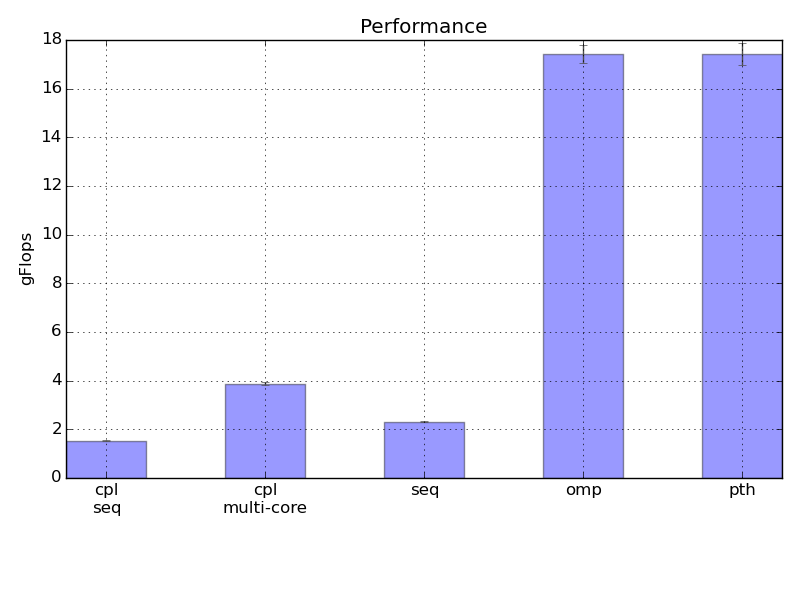
\includegraphics[width=\textwidth]{../cpl/report/per_no_reductions.png}
\end{frame}

\begin{frame}[fragile]
 \frametitle{Chapel: reductions}
\begin{verbatim}
for i in 1..p.N {
  for j in 1..p.M {
    var res = dst[i,j];
    var old = src[i,j];
    if (res < tmin) then tmin = res;
    if (res > tmax) then tmax = res;
...
\end{verbatim}
\end{frame}

\begin{frame}[fragile]
 \frametitle{Chapel: reductions}
\begin{verbatim}
r.maxdiff = max reduce [ij in ProblemSpace]
  abs(dst[ij] - src[ij]);

r.tmin = min reduce dst[ProblemSpace];
r.tmax = max reduce dst[ProblemSpace];
r.tavg = (+ reduce dst[ProblemSpace])
  / (p.N * p.M);
\end{verbatim}
\end{frame}

\begin{frame}[fragile]
 \frametitle{Chapel: custom reductions}
\begin{verbatim}
class heatReduction : ReduceScanOp {
  type eltType;
  var tmin: eltType = max(eltType);
  var tmax: eltType = min(eltType);
  var tsum: chpl__sumType(eltType);
\end{verbatim}
\end{frame}

\begin{frame}[fragile]
 \frametitle{Chapel: custom reductions}
\begin{verbatim}
proc accumulate(val: eltType)
  if (val < tmin) then tmin = val;
  if (val > tmax) then tmax = val;
  tsum += val;

proc combine(other: heatReduction)
  if (other.tmin < tmin) then
    tmin = other.tmin;
  if (other.tmax > tmax) then
    tmax = other.tmax;
  tsum += other.tsum;

proc generate()
  return new heatReductionResults(
    eltType, tmin, tmax, tsum);
\end{verbatim}
\end{frame}

\begin{frame}[fragile]
 \frametitle{Chapel: custom reductions}
\begin{verbatim}
r.maxdiff = max reduce [ij in ProblemSpace]
  abs(dst[ij] - src[ij]);

var reduction = heatReduction reduce
  dst[ProblemSpace];
r.tmin = reduction.tmin;
r.tmax = reduction.tmax;
r.tavg = reduction.tsum / (p.N * p.M);
\end{verbatim}
\end{frame}

\begin{frame}
 \frametitle{Chapel: w/reductions}
 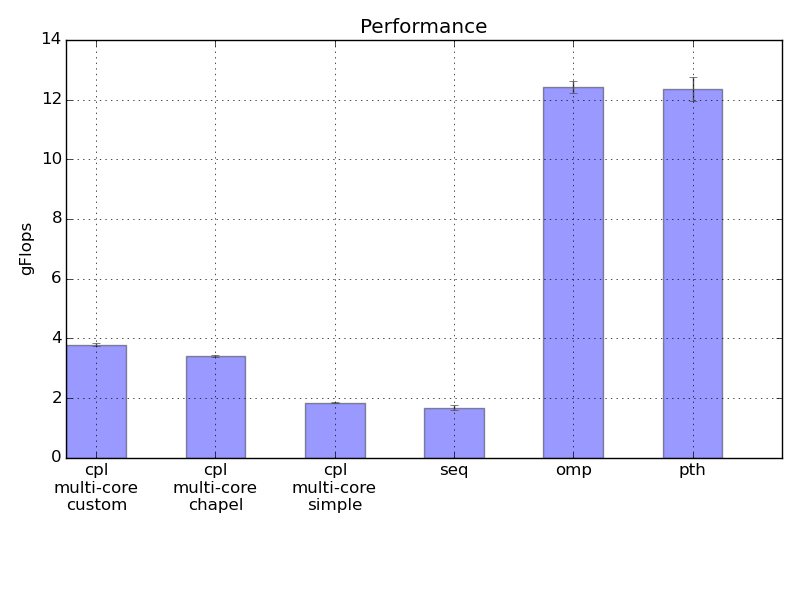
\includegraphics[width=\textwidth]{../cpl/report/per_with_reductions.png}
\end{frame}

\begin{frame}
 \frametitle{Questions?}
 (This time we mean it.)
\end{frame}

\end{document}
